\documentclass{article}
\usepackage[utf8]{inputenc}
\usepackage{geometry}
\usepackage{graphicx}
\usepackage{pgfplots}
\usepackage{verbatim}
\usepackage{amssymb}

\geometry{a4paper, left=2cm, right=2cm, top=1cm, bottom=2cm}

\begin{document}

\begin{minipage}{0.7\textwidth}
    \small \textbf{FÍSICA CONTEMPORÁNEA, GRUPO 8120}  \\
    \small {Facultad de Ciencias, Universidad Nacional Autónoma de México} \\
    \small {Profesor: Dr. Jesús Alberto Del Olmo Márquez (\texttt{jesus.delolmo@icat.unam.mx})} \\
    \small {Ayudante: M. Ismael Velázquez Gómez (\texttt{ismael.velazquez@icat.unam.mx})} \\
    \small {Fecha de entrega: 30 de Agosto de 2023} \\
    \small {Nombre completo: Andrés López González} \\
    \small {Tarea número 1}
\end{minipage}
\hfill
\begin{minipage}{0.12\textwidth}
    
\includegraphics[width=\linewidth]{logo_universidad}
\end{minipage}

\section*{Problema 1}

La función de movimiento \(x(t)\) de una partícula que se mueve a lo largo de un eje es: 
  \[x(t) = 4.0 - 6.0t^2\]
Con \(x\) en metros y \(t\) en segundos.
\begin{enumerate}
  \item ¿En qué momento y posición la partícula se detiene instantáneamente?\\
  \[
  x(t) = 4.0 - 6.0t^2, \frac{dx(t)}{dt} = v(x) = 0 \Rightarrow
  \frac{d}{dt}(4.0 - 6.0t^2) = 0\\\\
  -12.0t = 0
  t = 0s\\\\
  \]
  \[ x(0) = 4.0 - 6.0(0)^2 \Rightarrow x(0) = 4.0m \]
  

  \item ¿En qué momento la partícula pasa por el origen?\\
\textit{Por definición el origen en \(\mathbb{R}^2\) es la intersección del eje \textbf{x,y} tal que x(0) = 0. Demostraremos que \(x(0) \neq 0\) empezando con el tiempo donde t = 0s entonces...}
\[x(0) = 4.0 - 6.0(0)^2 \Rightarrow x(0) = 4.0m\]
\textit{Por otro lado debido a la naturaleza cuadrática de la ecuación tenemos dos valores para x(t) = 0}
\[
x(t) = 0 = 4.0 - 6.0(0)^2 \Rightarrow
6t^2 = 4 \Rightarrow |t| = \sqrt{\frac{2}{3}}
\therefore t = \pm \sqrt{\frac{2}{3}}s
\]
\textit{\textbf{Actualización: En clase se estableció que la respuesta era x(t) = 0 por lo que cuando pase por el origen será en:}}
\[ |x(t)| = 0 \textit{  en... }\sqrt{\frac{2}{3}} segundos \]

  
  \item Grafique \(x\) contra \(t\) para el intervalo de \(-5\) s a \(+5\) s.\\
  
\begin{center}
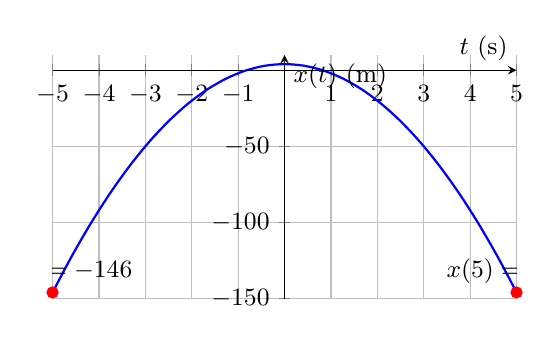
\begin{tikzpicture}
\small
\begin{axis}[
xlabel={$t$ (s)},
ylabel={$x(t)$ (m)},
xmin=-5, xmax=5,
ymin=-150, ymax=10,
grid=major,
xtick={-5, -4, -3, -2, -1, 0, 1, 2, 3, 4, 5},
ytick={-150, -100, -50, 0, 50, 100, 150},
width=10cm,
height=6cm,
axis lines=center, scale=0.7
]
\addplot[domain=-5:5, smooth, thick, blue]{4 - 6*x^2};
\addplot[mark=*, mark options={fill=red, draw=red}, only marks] coordinates {(5,-146)(-5,-146)};
\node[above] at (axis cs:5,-146) {$x(5)=-146$};
\node[above] at (axis cs:-5,-146) {$x(-5)=-146$};
\end{axis}
\normalsize
\end{tikzpicture}
\end{center}

  
  \item Si en el gráfico queremos desplazar la curva hacia la derecha, ¿debemos incluir el término \(+20t\) o el término \(-20t\) en la función de movimiento\\
  \textit{\textbf{Debemos sumar +20t}, esto debido a que las propiedades de las funciones dictaminan un desplazamiento a la derecha en su gráfica (incremento en los valores de su imagen) cuando les es sumado un valor positivo, cuando este no solo es un valor positivo sino también contiene a la variable entonces su desplazamiento se mostrará incrementado en forma de diagonal ascendente.}
  
  \item ¿Este desplazamiento aumenta o disminuye la posición en la que la partícula se detiene instantáneamente?
  \textit{\textbf{Aumenta.} Para observar este fenómeno calcularemos v(x) en la nueva ecuación para ver si el nuevo valor que obtendremos es positivo (desplazamiento a la derecha) o negativo (desplazamiento a la izquierda) de la forma siguiente:}
  \[\frac{d}{dt}(4.0 - 6.0t^2 + 20.0t) = v(t) = 0 \\\]
  \[-12.0t + 20.0 = 0 \Rightarrow 12.0t = 20.0 \\\]
  \[\therefore t = +\frac{20}{12}s = + \frac{5}{3}\]
\end{enumerate}

\section*{Problema 2}

La posición de una partícula que se mueve a lo largo del eje \(x\) en función del tiempo está determinada por la ecuación:

\[x(t) = Ct^2 - Bt^3\]

\noindent Donde \(x\) está en metros y \(t\) en segundos.

\begin{enumerate}
  \item ¿Cuáles son las unidades de las constantes \(C\) y \(B\)? Si sus valores numéricos son \(3.0\) y \(2.0\), respectivamente.
  \[
  [C][s^2] = [m] \Rightarrow [C] =  \frac{[m]}{[s^2]} \textit{  por otro lado B...  }
  [B][s^3] = [m] \Rightarrow [B] =  \frac{[m]}{[s^3]}
  \]
  
  \item ¿En qué momento, entre \(t_1 = 0.0s\) y \(t_2 = 4.0s\), la partícula alcanza su posición máxima? \\
  \[  x(t) = 3t^2 - 2t^3 \Rightarrow v(t) = \dot{x}(t) = 6t - 6t^2  \]
  \[ \textit{Puntos de pendiente 0:} \]
  \[ 6t (1-t) = 0 \therefore t_1 = 0 \cap t_2 = 1 \]
  \[ \textit{Máximos y mínimos:} \]
  \[ \ddot{x}(t) = 6 - 12t \]
  \[ \ddot{x}(0) = 6 \textit{  (Mínimo)  } \cap \textit{  }\ddot{x}(1) = -6 \textit{  (Máximo)  } \]
  \[ x(1) = 3(1)^2 - 2(1)^3 = 1m \]
  \[ \therefore \textit{La partícula alcanza su pósición máxima de 1m después de 1 segundo} \]
  
  
  \item En el mismo intervalo de tiempo, ¿qué distancia se mueve la partícula y cuál es su desplazamiento?\\
  \textit{La distancia la calculamos con la diferencia de posiciónes x(4) - x(0):}
  \[x(0) = 3(0)^2 - 2(0)^2 = 0\]
  \[x(4) = 3(4)^2 - 2(4)^2 = 48 - 128 = -80\]
  \[Distancia = |x_4-x_0| = |-80 - 0| = 80\]
  \textit{El desplazamiento con la suma de distancias en puntos importantes de la gráfica:}
  \[  Desplazamiento = \Delta x = x_4 - x_0 \Rightarrow -80 - 0 = -80m  \]
  \item Calcule su velocidad y aceleración para los tiempos \(t = \{1.0, 2.0, 3.0, 4.0\} \, \text{s}\).

\begin{center}
\(
v(x) = \dot{x}(t) = 6t - 6t^2 \Rightarrow a(x) = \ddot{x}(t) = 6 - 12t\\
\)
  \begin{tabular}{|c|c|c|c|}
    \hline
    Tiempo (\(t\)) & Velocidad (\(v(t)\)) & Aceleración (\(a(t)\)) \\
    \hline
    1.0 & 0 & -6 \\
    2.0 & -12 & -18 \\
    3.0 & -36 & -30 \\
    4.0 & -72 & -42 \\
    \hline
  \end{tabular}
\end{center}


\end{enumerate}


\section*{Problema 3}

Se deja caer un perno desde un puente en construcción a una altura de $90 \, \text{m}$ sobre un valle.

\begin{enumerate}
    \item ¿Cuánto tardará en iniciar el último 20\% de la caída? \\
  \textit{Usando la ecuación de movimiento:}
  \[
  y = y_0 + v_0t - \frac{gt^2}{2}
  \]
  \textit{podemos calcular el tiempo necesario para iniciar el último 20\% de la caída:}
  
  \[
  t = \sqrt{\frac{2\Delta y}{g}} = \sqrt{\frac{2 \cdot (0.80 \cdot 90)}{9.806}} \approx 3.83208 \, \text{s}
  \]
  
  \textit{Por lo tanto, el tiempo que tardará en iniciar el intervalo del 80 al 100\% es aproximadamente 3.83208 segundos, lo cual es congruente con el tiempo total del recorrido:}
  
  \[
  t_f = \sqrt{\frac{2\Delta y}{g}} = \sqrt{\frac{2 \cdot 90}{9.806}} \approx 4.2844 \, \text{s}
  \]
  
  \item ¿Cuál es su velocidad al comenzar el último 20\% de la caída? \\
  \textit{Considerando v(x) = gt entonces...}
  \[
  v_{\sqrt{\frac{144}{9.806}}} = 9.806 \cdot \sqrt{\frac{144}{9.806}} \approx 37.5774 \frac{m}{s}
  \]
  
  \item ¿Cuál es su velocidad al llegar al valle, justo antes de tocar el suelo? \\
  \textit{Ocupamos la misma ecuación de la velocidad pero evaluada en el instante final del recorrido}
  \[
  v_{\sqrt{\frac{180}{9.806}}} = 9.806 \cdot \sqrt{\frac{180}{9.806}} \approx 42.0128 \frac{m}{s}
  \]
\end{enumerate}

\section*{Problema 4}

Una bola de acero se deja caer desde el techo de un edificio y pasa por una ventana, tardando $0.125 \, \text{s}$ en pasar desde la parte superior hasta la parte inferior de la ventana, recorriendo una distancia de $1.20 \, \text{m}$. Llega a una acera y rebota pasando por la ventana, desde abajo hacia arriba en $0.125 \, \text{s}$. Suponga que el vuelo ascendente es idéntico al de la caída, pero en dirección contraria. El tiempo que la pelota pasa por debajo de la parte inferior de la ventana es de $2.00 \, \text{s}$. ¿Cuál es la altura del edificio?\\\\
\textit{Encontramos la velocidad de la bola al pasar por la ventana}
\[
v = \frac{d}{t} = \frac{1.2m}{0.125s} = 9.6 \frac{m}{s}
\] \\
\textit{Despejamos t de la fórmula de la velocidad final}
\[
v_f = v_0 - gt \Rightarrow t = \frac{v_0 - v_f}{g}
\] \\
\textit{Sustituimos...}
\[
\frac{(0-9.6)\frac{m}{s}}{-9.806\frac{m}{s^2}} = 0.978s
\] \\
\textit{Debido a que la pelota tarda 2 segundos desde la parte inferior de la ventana hasta su regreso, entonces se deduce que el tiempo que tardará desde el marco inferior de la ventana hasta el suelo será de 1 segundo. Sumamos 1 segundo con los 0.978 segundos previamente calculados para obtener el trayecto desde la parte superior del edificio hasta el suelo. Nuestro nuevo valor de t = 1.978 segundos}
\[
y = y_0 + v_0 + \frac{gt^2}{2} = 0 + 0 + \frac{gt^2}{2} = \frac{9.806\frac{m}{s^2} \cdot 1.978^2s^2}{2} = \frac{38.40}{2} = 19.20m
\]
\textit{La altura del edificio es 19.20m}

\section*{Problema 5}



\noindent A partir de la siguiente ecuación:

\[
\frac{d}{dt}F(t) = \frac{d}{dt}[G(t) \cdot H(t)] = G(t) \frac{d}{dt}H(t) + H(t) \frac{d}{dt}G(t) \quad \text{(1)}
\]

\noindent que indica la derivada del producto de dos funciones, demuestre que la derivada del cociente de dos funciones está determinada por:

\[
\frac{d}{dt}\left(\frac{G(t)}{H(t)}\right) = \frac{H(t)\frac{d}{dt}G(t) - G(t)\frac{d}{dt}H(t)}{H^2(t)} \quad \text{(2)}
\]

\textit{Usamos reglas más básicas de la derivada como la del producto que se nos es indicada, regla de la potencia y axioma del inverso de una función}\\\\
\(
\frac{d}{dt}\left(\frac{G(t)}{H(t)}\right) \\\\
= \frac{d}{dt}\left(G(t) \cdot \frac{1}{H(t)}\right) \\\\
= \frac{d}{dt}\left(G(t) \cdot H(t)^{-1}\right) \\\\
= G(t) \cdot \frac{d}{dt}\left(H(t)^{-1}\right) + H(t)^{-1} \cdot \frac{d}{dt}\left(G(t)\right) \\\\
= G(t) \cdot \left(-H(t)^{-2} \cdot \frac{d}{dt}\left(H(t)\right)\right) + H(t)^{-1} \cdot \frac{d}{dt}\left(G(t)\right) \\\\
= -\frac{G(t)}{H(t)^2} \cdot \frac{d}{dt}\left(H(t)\right) + \frac{1}{H(t)} \cdot \frac{d}{dt}\left(G(t)\right) \\\\
= \frac{H(t)}{H(t)^2} \cdot \frac{d}{dt}\left(G(t)\right) - \frac{G(t)}{H(t)^2} \cdot \frac{d}{dt}\left(H(t)\right) \\\\
= \frac{H(t) \cdot \frac{d}{dt}\left(G(t)\right) - G(t) \cdot \frac{d}{dt}\left(H(t)\right)}{H(t)^2} \\\\
\) \\

\noindent Utilizando este resultado, calcule la derivada de las siguientes funciones:

\begin{enumerate}
    \item \(x(t) = \frac{t^3}{(t + \beta)^2}\), donde \(\beta\) es una constante. \\\\
    \( %Apertura 1
    \frac{dx(t)}{dt}
    = \frac{(t + \beta)^2\frac{d}{dt}t^3 - t^3\frac{d}{dt}(t + \beta)^2}{(t + \beta)^{2^2}}
    = \frac{3t^2 \cdot (t + \beta)^2 - 2t^3 \cdot (t + \beta)}{(t + \beta)^4}
    = \frac{3t^2 \cdot (t + \beta) - 2t^3}{(t + \beta)^3}
    = \frac{3t^3 + 3t^2\beta - 2t^3}{(t + \beta)^3}
    = \frac{t^3 + 3t^2\beta}{(t + \beta)^3}
    = \frac{t^2(t + 3\beta)}{(t + \beta)^3}
    \) %Cerradura 1
    
    \item \(f(y) = \frac{3ay^2 + b}{cy^3 + y + d}\), donde \(a\), \(b\), \(c\), y \(d\) son constantes. \\\\
    \( %Apertura 2
    \frac{df(y)}{dy}
    = \frac{(cy^3 + y + d)\frac{d}{dy}(3ay^2 + b) - (3ay^2 + b)\frac{d}{dy}(cy^3 + y + d)}{(cy^3 + y + d)^2} = \frac{6ay \cdot (cy^3 + y + d) + (-3ay^2 - b) \cdot (3cy^2 + 1)}{(cy^3 + y + d)^2} \\\\
    = \frac{6acy^4+6ay^2+6ady-9acy^4-3ay^2-3bcy^2-b}{(cy^3+y+d)^2}
    = \frac{-3acy^4+3ay^2+6ady-3bcy^2-b}{(cy^3+y+d)^2}
    \) %Cerradura 2

%    \item \(v(x) = \frac{e^{\alpha x}}{\alpha^2 (\alpha x - 1)}\), donde \(\alpha\) es una constante. \\\\ \(\frac{dv(x)}{dx} = \frac{(\alpha^2 (\alpha x - 1))\frac{d}{dx}(e^{\alpha x}) - (e^{\alpha x})\frac{d}{dx}(\alpha^2 (\alpha x - 1))}{(\alpha^2 (\alpha x - 1))^2} \textit{tenemos que  }      \alpha^2(\alpha x -1) = \alpha^3x-\alpha^2 \Rightarrow \\\\ \frac{(\alpha^2 (\alpha x - 1))\frac{d}{dx}(e^{\alpha x}) - (e^{\alpha x})\frac{d}{dx}(\alpha^2 (\alpha x - 1))}{(\alpha^2 (\alpha x -  1))^2} = \frac{(\alpha^3x-\alpha^2)\frac{d}{dx}(e^{\alpha x}) - (e^{\alpha x})\frac{d}{dx}(\alpha^3x-\alpha^2)}{(\alpha^3x-\alpha^2)^2} = \frac{\alpha(\alpha^3x-\alpha^2)e^{\alpha x} - (\alpha^3 \cdot 1)e^{\alpha x}}{(\alpha^3 x - \alpha^2)^2} = \frac{(\alpha^4x-\alpha^3)e^{\alpha x} - \alpha^3e^{\alpha x}}{(\alpha^3 x - \alpha^2)^2} \\ \)

    \item \(v(x) = \frac{e^{\alpha x}}{\alpha^2} \cdot (\alpha x - 1) \), donde \(\alpha\) es una constante. \\\\
    \( %Apertura 3
    \frac{dv(x)}{dx}
    = \frac{d}{dx}(\frac{e^{\alpha x}}{\alpha^2})(\alpha x-1) + \frac{e^{\alpha x}}{\alpha^2} \cdot \frac{d}{dx}(\alpha x-1)
    = \frac{\frac{d(e^{\alpha x)}}{dx} \cdot \alpha^2 - e^{\alpha x} \cdot \frac{d(\alpha^2)}{dx}}{\alpha^4} \cdot (\alpha x-1) + \frac{e^{\alpha x}}{\alpha^2} \cdot (\alpha-0)\\\\
    = \frac{\alpha^3e^{\alpha x}-(0)e^{\alpha x}}{\alpha^4} \cdot (\alpha x-1) + \frac{e^{\alpha x}}{\alpha}
    = \frac{\alpha^3e^{\alpha x}(\alpha x-1)}{\alpha^4} + \frac{e^{\alpha x}}{\alpha}
    = \frac{e^{\alpha x}(\alpha x-1)}{\alpha} + \frac{e^{\alpha x}}{\alpha}
    = \frac{e^{\alpha x}(\alpha x-1) + e^{\alpha x}}{\alpha}
    = \frac{e^{\alpha x}((\alpha x-1) + 1)}{\alpha} \\\\
    = \frac{e^{\alpha x}\alpha x}{\alpha}
    = e^{\alpha x}x
    \) %Cerradura 3
    
    \item \(S(h) = t + \frac{c^2h^2}{1+\sqrt{1-(k+1)c^2h^2}}\), donde \(c\), \(k\), y \(t\) son constantes. \\
    \( %Apertura 4
    \frac{dS(h)}{dh}
    = \frac{dt}{dh} + \frac{d}{dh}(\frac{c^2h^2}{1+\sqrt{1-kc^2h^2+c^2h^2}})
    = 0 + \frac{\frac{d(c^2h^2)}{dh} \cdot (1+\sqrt{1-kc^2h^2+c^2h^2}) - c^2h^2 \cdot \frac{d}{dh}(1+\sqrt{1-kc^2h^2+c^2h^2})}{(1+\sqrt{1-kc^2h^2+c^2h^2})^2}\\\\
    = 0 + \frac{\frac{d(c^2h^2)}{dh} \cdot (1+\sqrt{1-kc^2h^2+c^2h^2}) - c^2h^2 \cdot (\frac{d(1)}{dh}+\frac{d}{dh}(1-kc^2h^2+c^2h^2)^{1/2})}{(1+\sqrt{1-kc^2h^2+c^2h^2})^2} \\\\
    = \frac{\frac{d(c^2h^2)}{dh} \cdot (1+\sqrt{1-kc^2h^2+c^2h^2}) - c^2h^2 \cdot (0 + \frac{1}{2} \cdot (1-kc^2h^2+c^2h^2)^{-1/2} \cdot \frac{d(1-kc^2h^2+c^2h^2)}{dh} )}{(1+\sqrt{1-kc^2h^2+c^2h^2})^2}\\\\
    = \frac{\frac{d(c^2h^2)}{dh} \cdot (1+\sqrt{1-kc^2h^2+c^2h^2}) - c^2h^2 \cdot (\frac{1}{2\sqrt{1-kc^2h^2+c^2h^2}} \cdot (0-2kc^2h+2c^2h))}{(1+\sqrt{1-kc^2h^2+c^2h^2})^2}\\\\
    = \frac{2c^2h \cdot (1+\sqrt{1-kc^2h^2+c^2h^2}) - c^2h^2 \cdot (\frac{2(c^2h-kc^2h)}{2\sqrt{1-kc^2h^2+c^2h^2}})}{(1+\sqrt{1-kc^2h^2+c^2h^2})^2}\\\\
    = \frac{2c^2h+2c^2h\sqrt{1-kc^2h^2+c^2h^2} - \frac{(c^4h^3-kc^4h^3)}{\sqrt{1-kc^2h^2+c^2h^2}}}{(1+\sqrt{1-kc^2h^2+c^2h^2})^2} \textit{  racionalizando   } \frac{(c^4h^3-kc^4h^3)}{\sqrt{1-kc^2h^2+c^2h^2}}
    = \frac{(c^4h^3-kc^4h^3)\sqrt{1-kc^2h^2+c^2h^2}}{1-kc^2h^2+c^2h^2}\\\\
    = \frac{2c^2h+2c^2h\sqrt{1-kc^2h^2+c^2h^2} - \frac{(c^4h^3-kc^4h^3)\sqrt{1-kc^2h^2+c^2h^2}}{1-kc^2h^2+c^2h^2}}{(1+\sqrt{1-kc^2h^2+c^2h^2})^2}
    \) %Cerradura 4
\end{enumerate}

\end{document}
